\item\subquestionpointscoding{5} \textbf{Semi-supervised EM Implementation.}
Now we will consider both the labelled and unlabelled examples (a total of $\nexp + \tilde{\nexp}$), with 5 labelled examples per cluster. We have provided starter code for splitting the dataset into matrices \texttt{x} and \texttt{x\_tilde} of unlabelled and labelled examples respectively. Add to your code in \texttt{src/semi\_supervised\_em/gmm.py} to implement the modified EM algorithm, and run it on the dataset until convergence.

To verify a correct implementation, consider creating a plot for each trial, as done in the previous sub-question.

Your plots should look similar to the following (your plots are not graded):

  \begin{figure}[H]
    \centering
    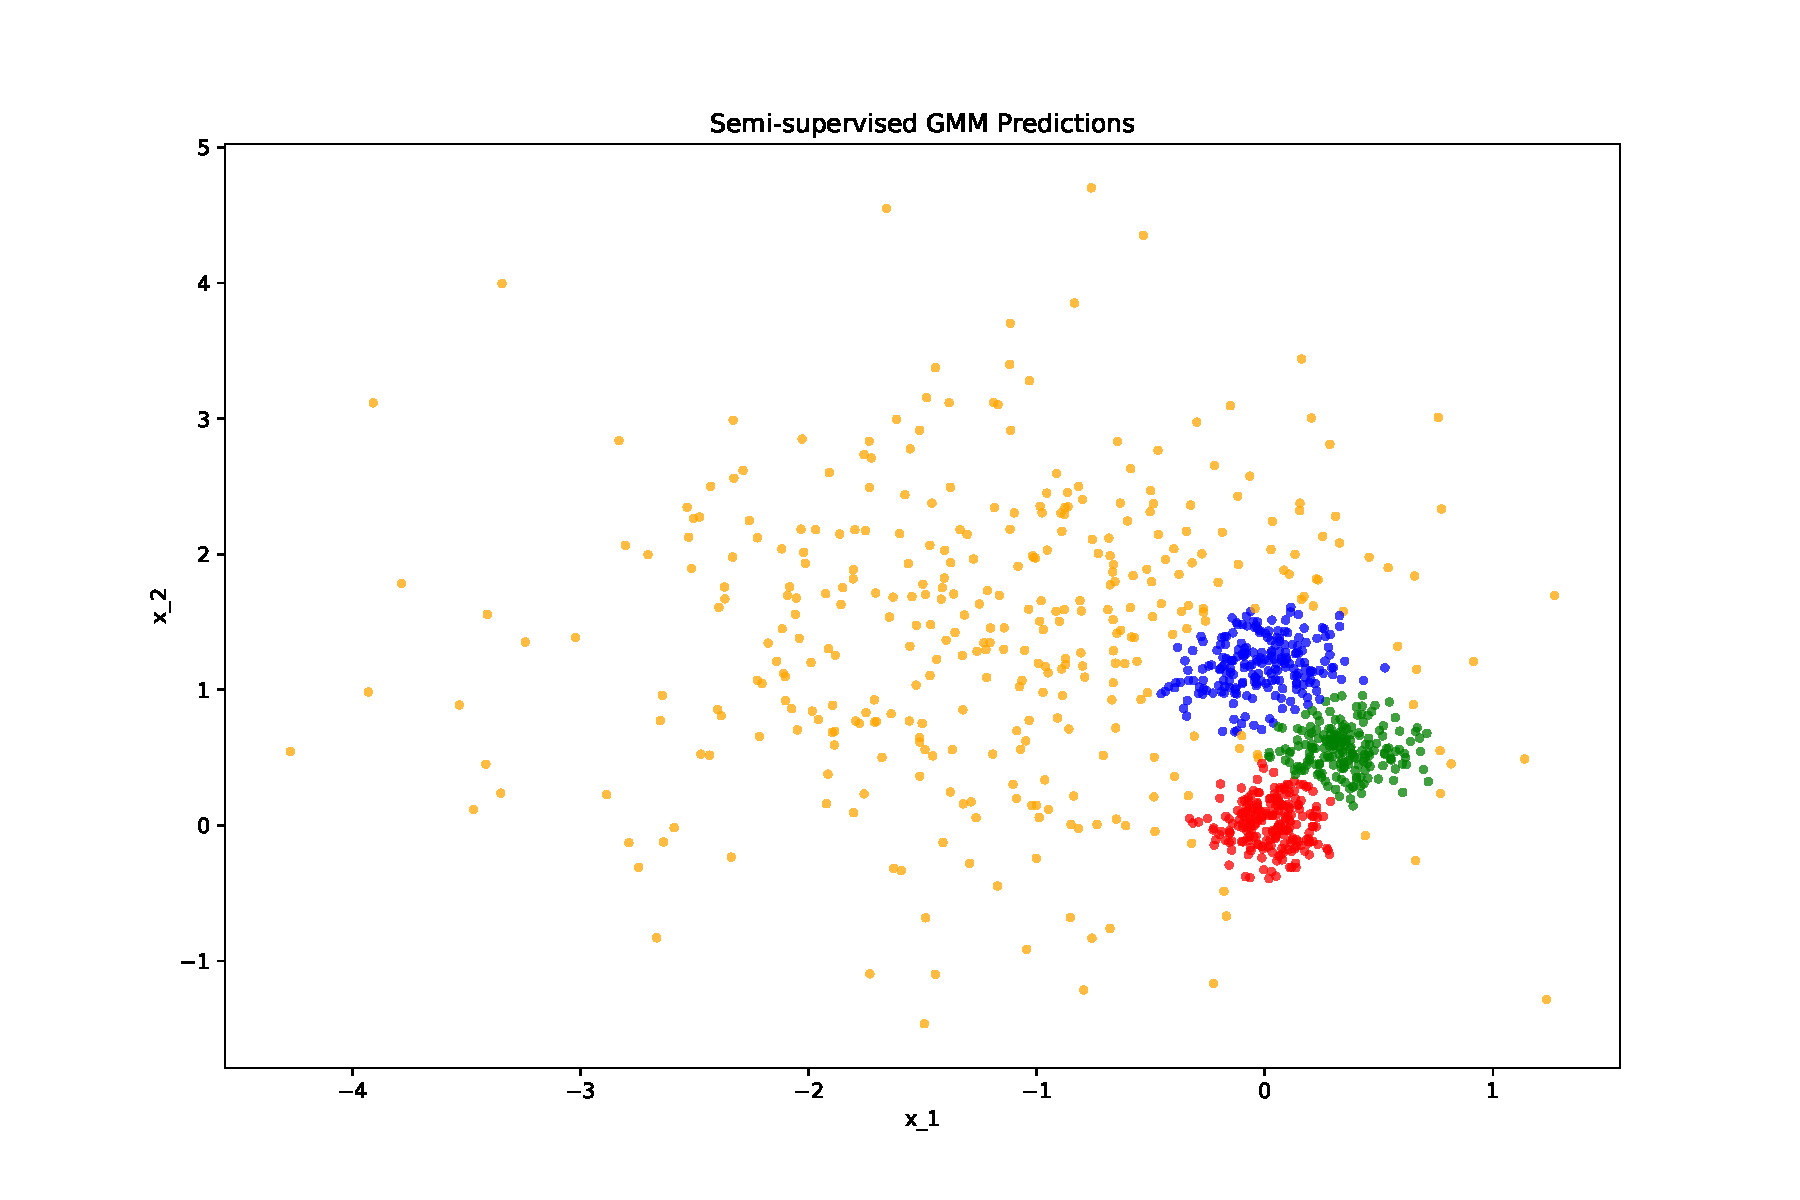
\includegraphics[width=0.3\textwidth]{semi_supervised_em/pred_ss_0.pdf}
    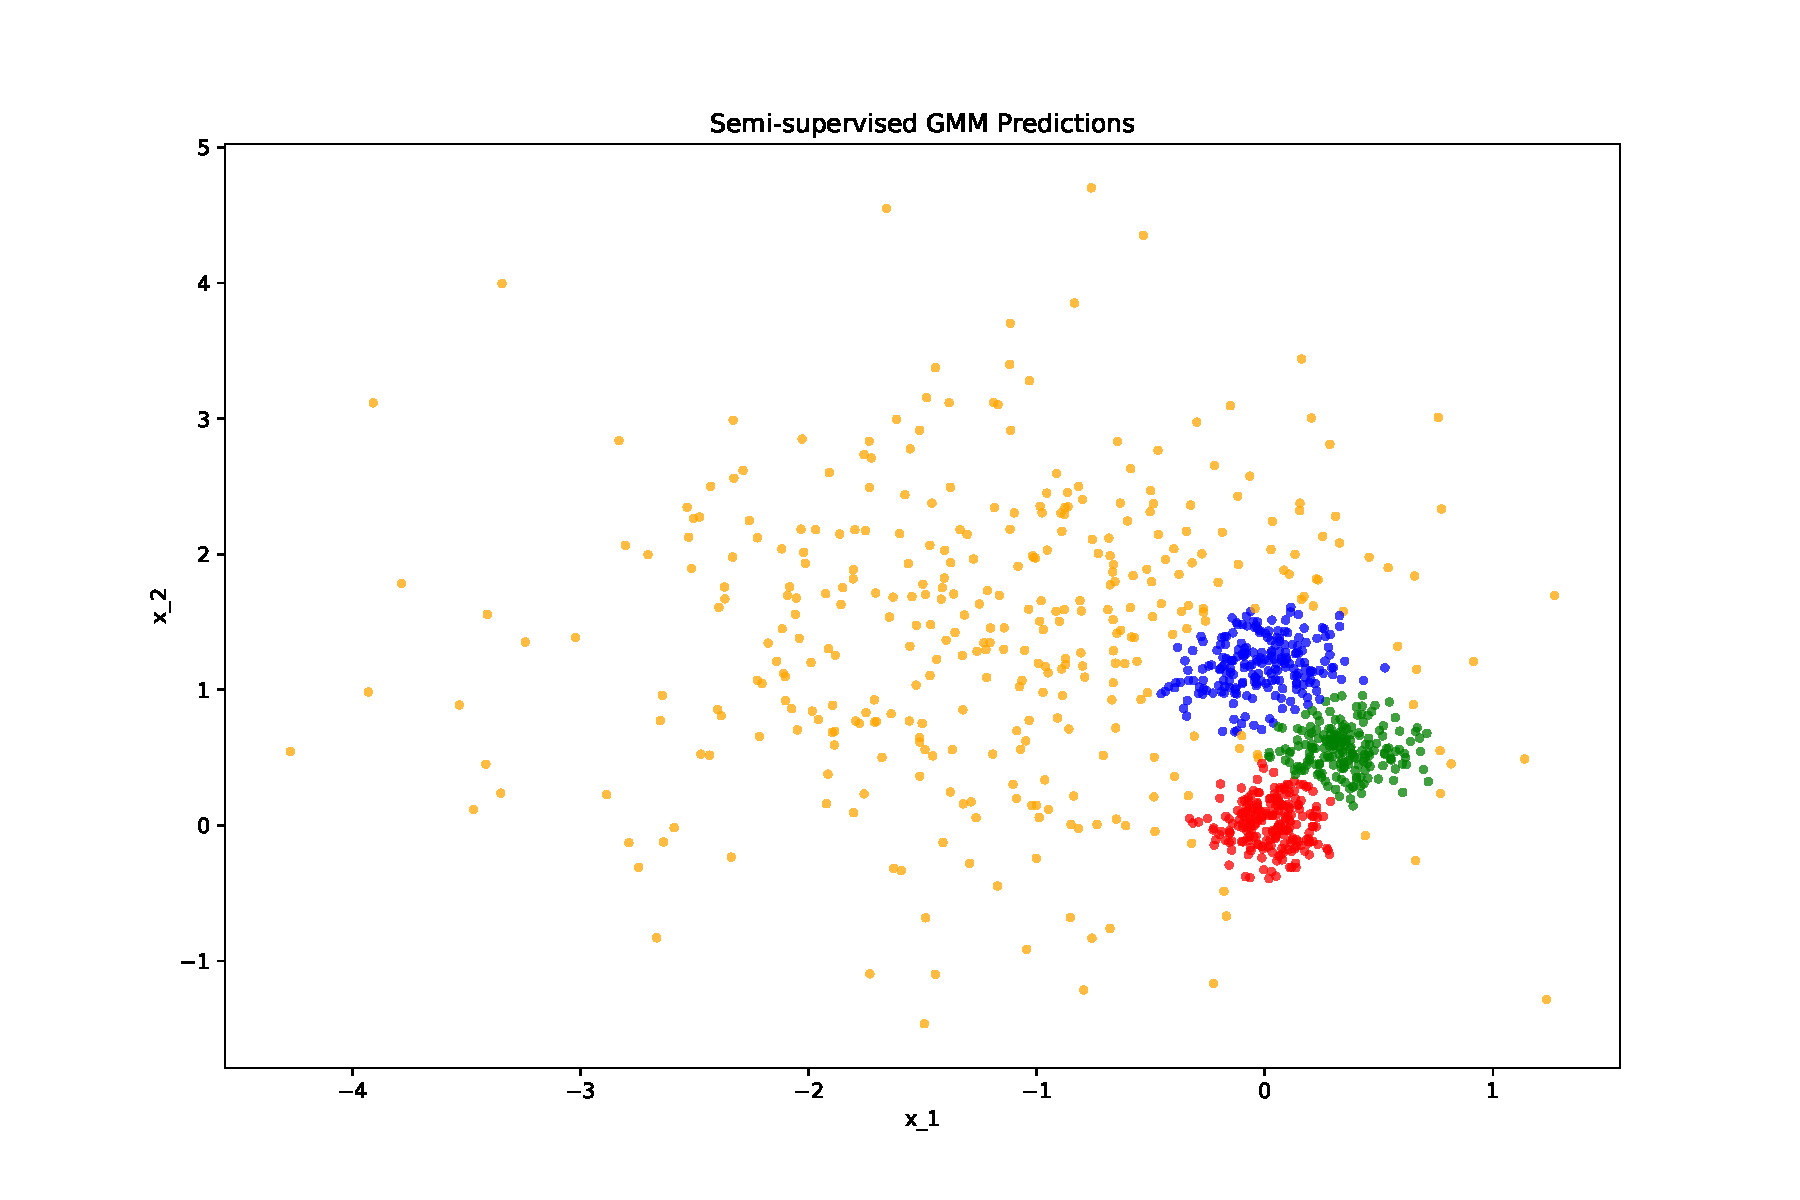
\includegraphics[width=0.3\textwidth]{semi_supervised_em/pred_ss_1.pdf}
    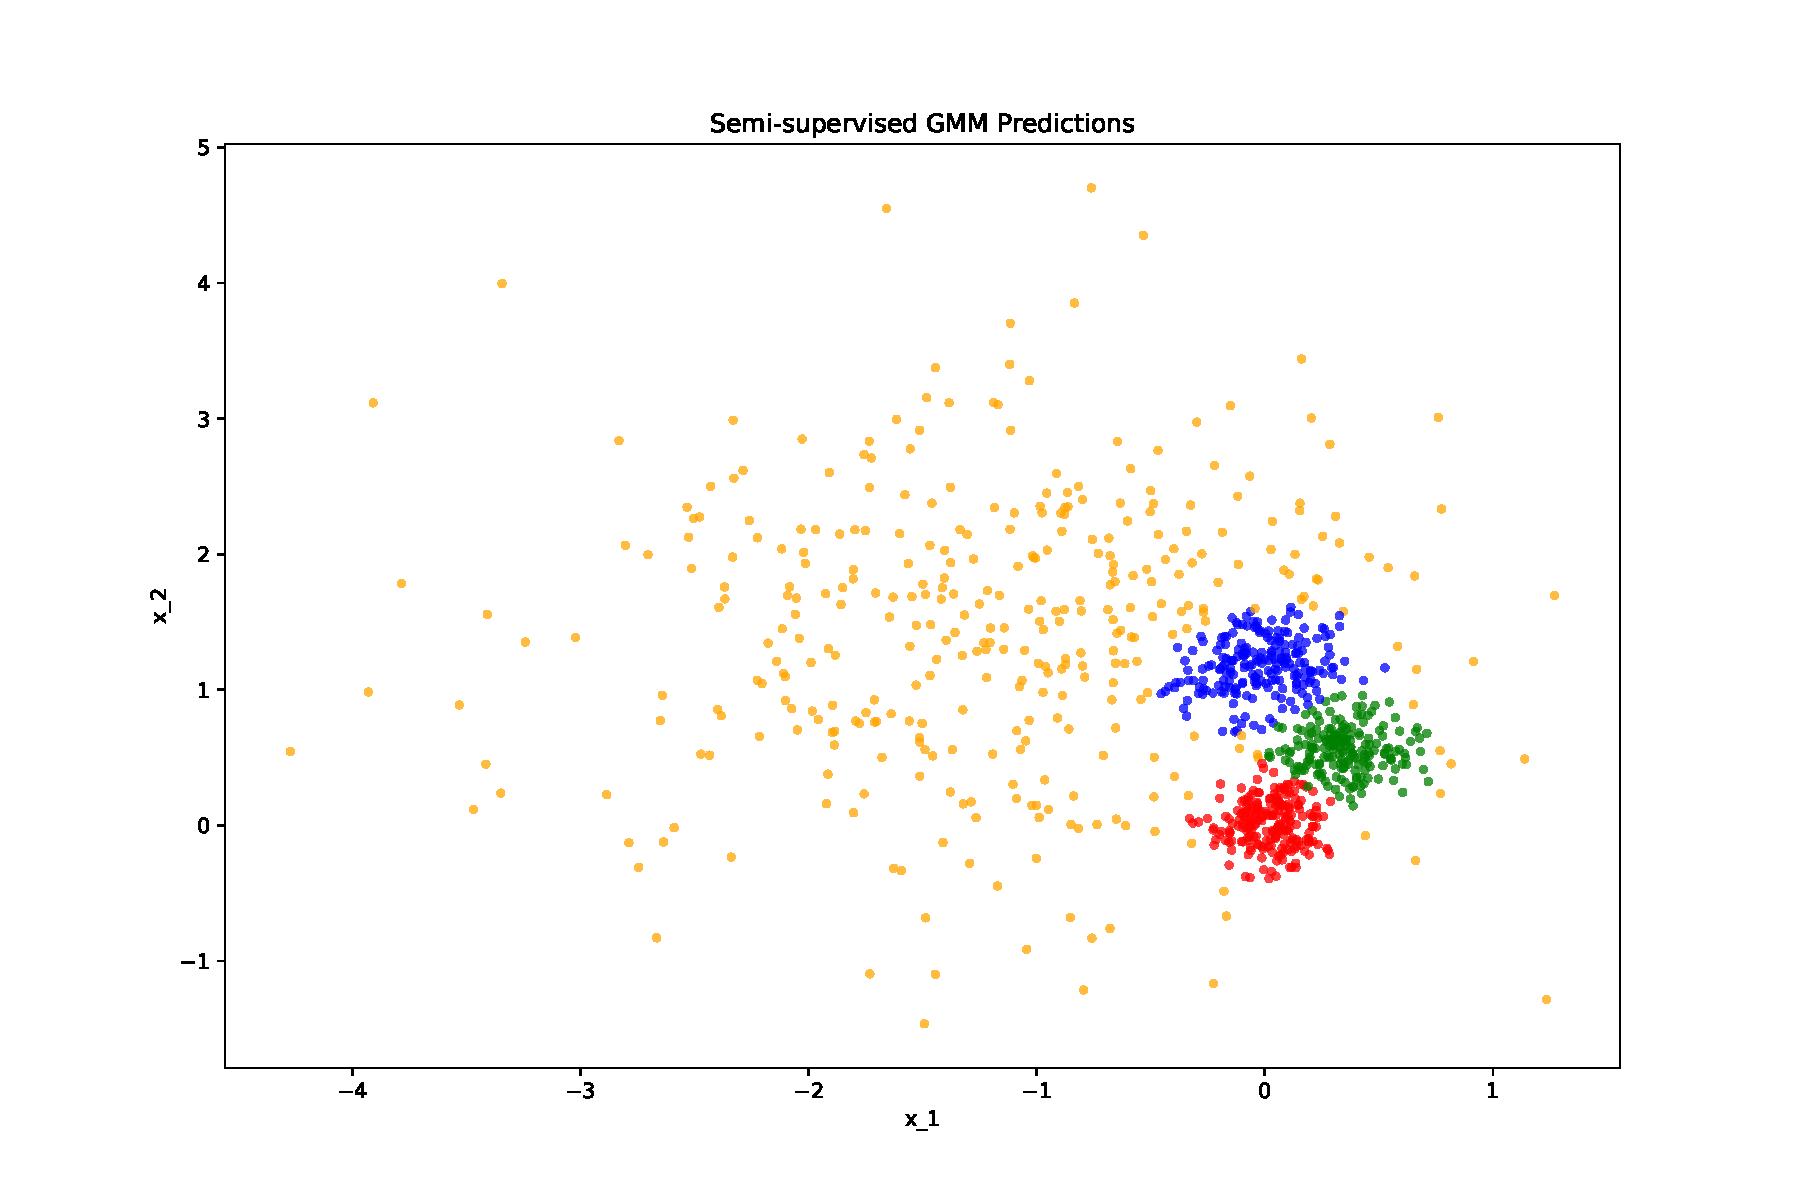
\includegraphics[width=0.3\textwidth]{semi_supervised_em/pred_ss_2.pdf}
    \caption{Predictions made by GMM model with semi-supervised EM.}
  \end{figure}
